\documentclass[conference]{IEEEtran}  % Don't change

% You can add external packages
\usepackage{cite} % This is a package that modifies the way citations are handled and formatted, particularly useful for those writing academic or research papers where references are a key component.
\usepackage{amsmath,amssymb,amsfonts}  % packages provided by the American Mathematical Society (AMS), each offering various features particularly useful for typesetting mathematical content. 
\usepackage{algorithmic} % This package is used for typesetting algorithms
\usepackage{graphicx} % It adds support for including graphics in the document
\usepackage{textcomp} % Extra support for the text companion fonts
\usepackage{xcolor} % support for colored text and colored boxes in LaTeX documents.
\usepackage{pdfpages}


% Add more external upackages if you need
% \usepackage{}

\def\BibTeX{{\rm B\kern-.05em{\sc i\kern-.025em b}\kern-.08em
    T\kern-.1667em\lower.7ex\hbox{E}\kern-.125emX}}   % Don't change
%\def\BibTeX defines a new command named \BibTeX

% add a new theorem if you need:
% \newtheorem{theorem}{Theorem}


\begin{document}

\title{ECM2427: Literature Review on [ARM vs x86 Architectures in Cloud Computing]}


\author{\IEEEauthorblockN{Anonymised Author} % Don't change - don't add you name, email, SID - any identifiable information here
}


% to generate the title of the paper
\onecolumn
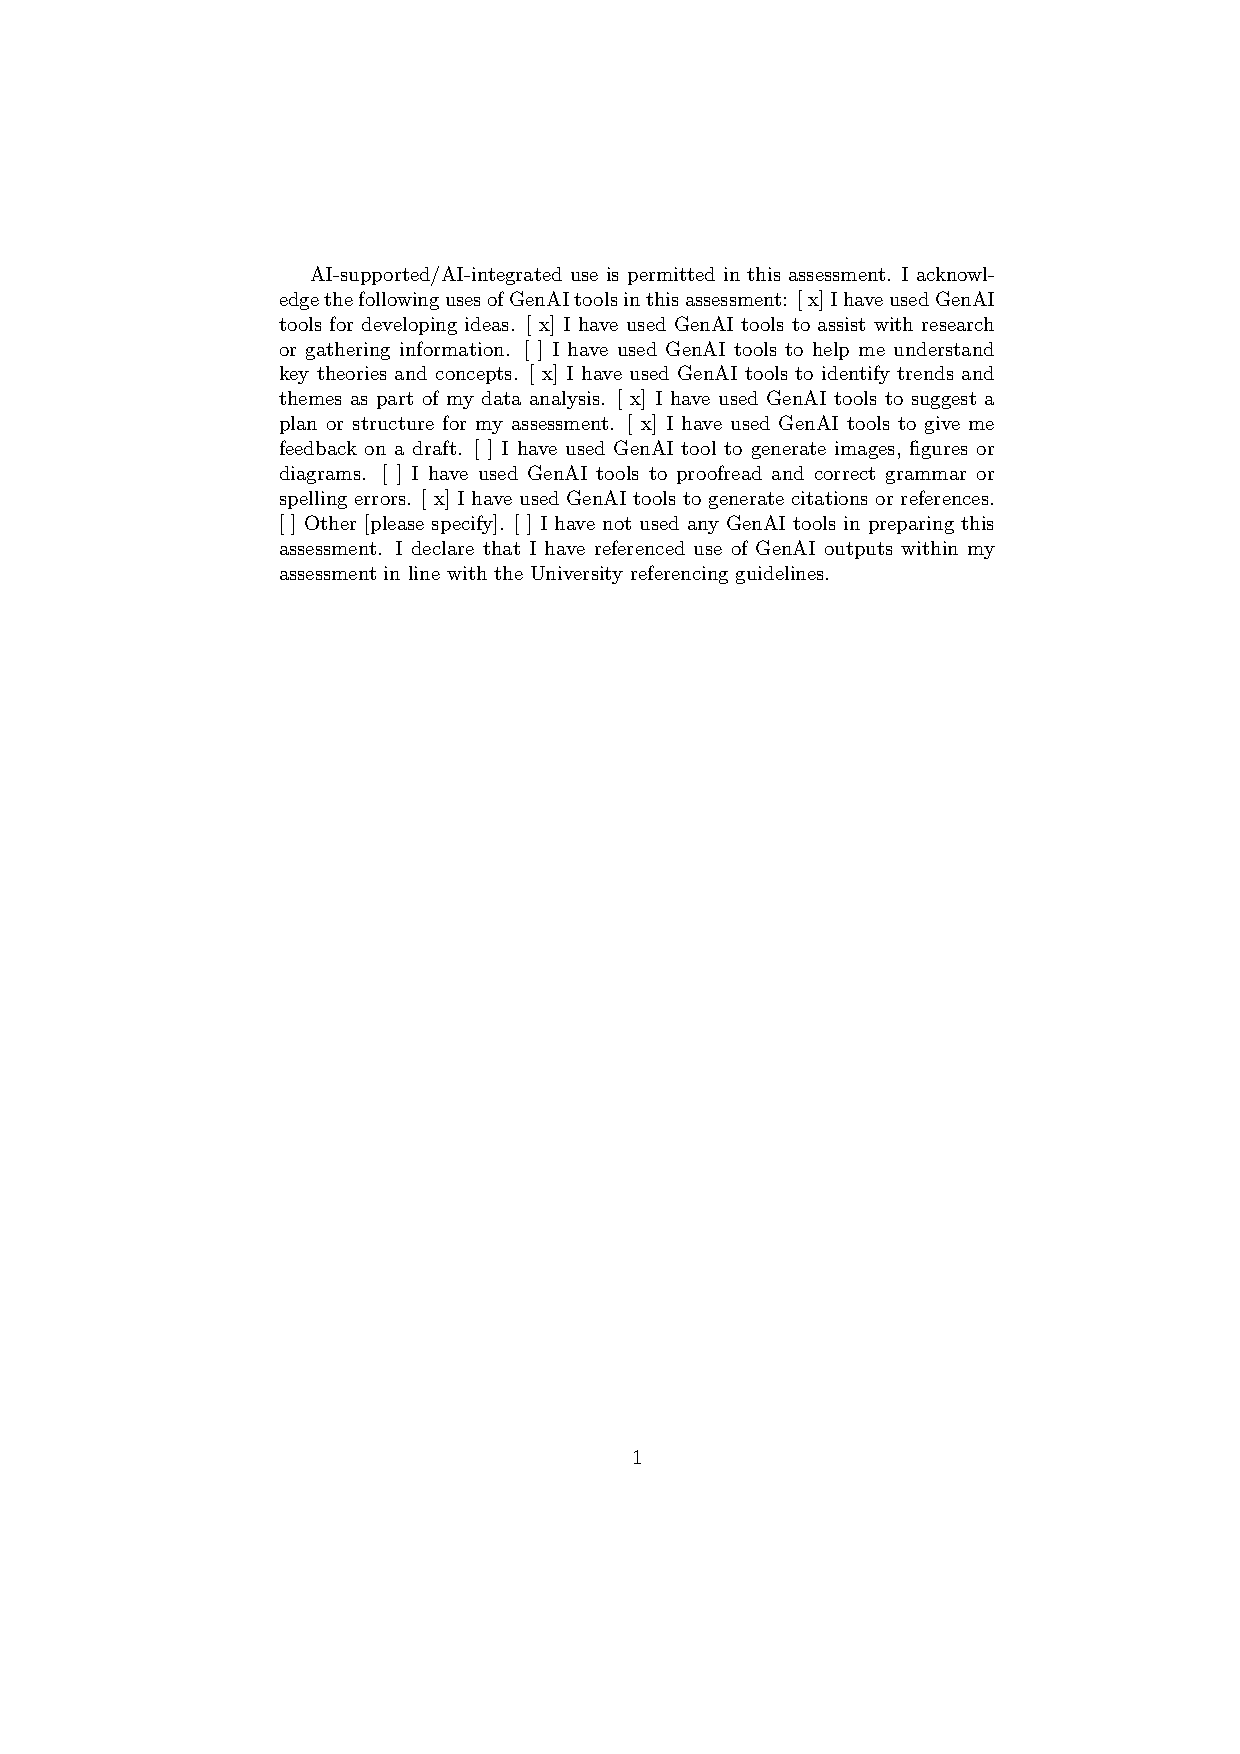
\includepdf[pages=-, fitpaper=true]{ai.pdf}
\twocolumn
\maketitle  % Don't change


\section{Introduction} % Don't change

Cloud computing has become an essential paradigm in modern computing and the digital age.
Cloud computing relies heavily on high-performance computing (HPC) systems within data centres around the world.
Traditionally, servers in these data centres have utilised the x86 architecture. However, with ever-increasing demands for scalability, energy efficiency, and cost-effectiveness, a shift away from x86 is being driven.

This literature review seeks to examine the growing role of ARM-based processors in cloud computing, an architecture initially prominent in embedded systems and mobile devices, which is now increasingly seen in place of x86 processors.
The purpose of this review is to analyse the key factors driving this shift to ARM-based processors, including their performance characteristics, advantages in energy efficiency, and challenges related to software support.

This review is organised thematically, covering the following key areas: 1) ARM Architecture and Cloud Adoption, 2) Performance Considerations, 3) Energy Efficiency and Sustainability, and 4) Software Ecosystem and Compatibility.
This thematic approach allows for a focused and in-depth analysis of each of these critical aspects.

The scope of this review is delimited to recent advancements and trends in cloud computing architectures.
While the historical context of both architectures is acknowledged, the primary emphasis is on current research and developments within the last decade.

The review concentrates on peer-reviewed academic publications, industry reports, and technical documentation from reputable sources to ensure the validity and reliability of the information presented. In some cases, articles from reputable magazines are also included to provide context or illustrate current trends.

The methodology for selecting and analysing sources involved a systematic search of academic databases (e.g., IEEE Xplore, ACM Digital Library), conference proceedings, and industry publications. Keywords such as "ARM server," "cloud computing architecture," "ARM vs. x86," and "data center energy efficiency" were used to identify relevant literature. The analysis of the selected sources involved summarizing key findings, comparing and contrasting different perspectives, and identifying trends and gaps in the literature.


\section{Review} % Don't change

My review structure is [\textbf{Thematic}]
\subsection{ARM Architecture and Cloud Adoption}
What fundamentally makes ARM different to x86 is their instruction set architectures (ISAs).
The x86 architecture uses a Complex Instruction Set Computing (CISC) design, distinguished by its ability to execute complex instructions.
This design aims to complete complex tasks in one instruction rather than needing multiple. 
In contrast ARM employs a Reduced Instruction Set Computing (RISC) architecture, this focuses on executing simpler instructions, emphasising power efficiency over clock speed. \cite{ARM_RISC_vs_x86_SISC}
It was found that only 20\% of instructions defined in CISC were commonly used, with 80\% being rarely used, therefore RISC became a popular choice. \cite{instructions_CISC_vs_RISC}

ARM established itself as a great architecture for mobile and ubiquitous devices, due to it's power efficiency, and that these devices didn't need as much processing power as a consumer desktop or laptop.
This emphasis on efficiency allowed for an extended battery life, compact design, and a cooler device \cite{furber1988advantages}.
However, ARM's applicability has expanded significantly beyond its origins in mobile and embedded systems. Driven by the increasing demands for scalable and energy-efficient computing solutions in data centres \cite{ARM_to_server}, the ARM architecture is increasingly penetrating the server domain and assuming a growing role in cloud computing. Cloud providers are drawn to ARM's potential to reduce operational costs associated with power consumption and cooling, particularly in hyperscale data centres where energy efficiency is paramount \cite{datacentre_energy}. 
A notable example of this shift from x86 to ARM in servers is Amazon Web Services (AWS) and their development of the Graviton family of ARM-based processors.
These processors, while not able to handle the same workload intensity as a traditional x86 processor, have greater cost savings on tasks such as video transcoding or terabyte scale sorting \cite{AWS_ARM}.

\subsection{Performance Considerations}
Performance is a critical factor in cloud computing, many websites are hosted in the cloud so having a smooth, responsive user experience (UX) is essential for companies to maintain customer loyalty. 

ARM and x86 architectures differ in their fundamental design philosophies, which can lead to differences in performance characteristics.
The variations between the two architectures can differ significantly depending on the workload.
In a study comparing HPC for ARM and x86, two clusters were made for each architecture \cite{arm_x86_clusters}.
In common benchmarking programs, ARM processors significantly lagged behind x86 processors, not only due to limited on-chip resources but also due to ARM's RISC architecture requiring extensive memory accesses. 
Applications like database operations can be very memory intensive, showing ARM's limitations as x86 server processors like Intel's Xeon range outperform even the latest ARM processors in a database context \cite{arm_database}. 

However, ARM doesn't always lose to x86.
ARM systems for a particular application, the Sieve of Eratosthenes, actually surpass x86 in terms of performance \cite{armBetter}. 
ARM doesn't try to sell itself as the fastest architecture but as one of if not the most efficient architectures. 
Many major cloud infrastructure providers offer ARM-based cloud instances, claiming better scalability, more predictable performance, and a lower cost compared to x86-based instances. \cite{ArmCloudComputing}




\subsection{Energy Efficiency and Sustainability}
One of the major advantages of ARM over x86 is it's energy efficiency, stemming from its RISC design, involving a simpler instruction set, requiring fewer transistors and consuming less power for each operation.

A study by NTT DATA demonstrated that an ARM server consumed 37\% less power than an x86 server while delivering roughly three times the processing power in a prime number search \cite{PrimeArmEfficiency}
This resulted in a roughly 4.8 times increase in performance for watt. 
This increase in performance while consuming less power is due to ARM better scalability. 
The two Intel Xeon Gold 6330 processors in the study each had 28 cores and hyper-threading enabled, totalling 56 cores and 112 threads across the two processors. 
In contrast, the ARM server used a single Ampere M128-30 processor featuring 128 cores each with a single thread. 
The higher core count and simpler threading model demonstrates ARM's superior scalability, while remaining more power efficient.

Data centres have seen a massive increase in energy consumption with advancements in cloud and edge computing, expected to account for 3.2\% of global carbon emissions in 2025 and 14\% in 2040 \cite{datacentreEnergy}. 
As demand for cloud computing increases for example, AI workloads, the need for more power efficient processing is only growing.
By increasing the performance per watt of processors, less energy is consumed and less cooling is needed, creating overall more efficient data centres.

\subsection{Software Ecosystem and Compatibility}
A major concern with the move away from x86 is leaving behind its mature software ecosystem.
The x86 architecture became the preferred choice for servers, which led to the development of a rich and extensive software ecosystem. 
Comparatively, ARM has been used in servers for much less time, which could lead one to think that its software ecosystem would be far behind x86's.

However, recent work suggests that the ARM software ecosystem is rapidly maturing, particularly in the context of HPC \cite{armEco}.
Research projects like the European Mont-Blanc, the Japanese Post-K, and the UK's GW4/EPSRC have focused on deploying ARM-based clusters, driving development and optimisation of software for the architecture. 
A Study from 2017 tested ARM's software ecosystem for HPC, finding no major obstacles, supporting all the available parallelism \cite{armEco}.

As ARM's interest and development has only grown, it is clear the software ecosystem for ARM is not lacking, and sees continual improvement. The recent adoption of ARM processors in consumer laptops, such as MacBooks or devices running Windows on ARM, requiring support for a broad range of applications, further demonstrates the ecosystem's expanding capabilities \cite{armLaptop}.
However, the software ecosystem has not been fully matured, Amazon received a large number of returns of ARM-based Microsoft surface laptops as people struggled with certain software lacking support natively, and instead having to be emulated, greatly reducing performance \cite{windowsOnArmWoes}.



\section{Conclusion} % Don't change
This literature review has examined the evolving role of ARM architecture in cloud computing, contrasting it with the traditional dominance of x86. The fundamental differences in their instruction set architectures (ISAs), with ARM's RISC design prioritising power efficiency and x86's CISC design historically focusing on performance, have led to distinct advantages and disadvantages for each in various cloud workloads.\cite{ARM_RISC_vs_x86_SISC} \cite{instructions_CISC_vs_RISC}

The increasing demand for scalable and energy-efficient solutions in cloud data centres has driven the adoption of ARM-based servers, as cloud providers seek to reduce operational costs and improve sustainability \cite{datacentre_energy}. While x86 processors have traditionally held a performance edge in certain compute-intensive tasks, ARM processors are demonstrating competitive performance, particularly in terms of price-performance and energy efficiency, and are well-suited for many cloud-native applications \cite{ArmCloudComputing}.

Overall, the literature suggests that ARM architecture presents a compelling alternative to x86 in cloud computing. Its superior energy efficiency offers significant economic and environmental benefits, and its performance capabilities are rapidly improving. Continued advances in ARM technology and software optimisation will likely further accelerate its adoption in the cloud.
While x86 remains a dominant force, particularly in legacy systems and certain HPC applications \cite{arm_database}, ARM is setup to be an increasingly significant part of the cloud computing industry.

% This command sets the style in which the bibliography is formatted. You must use IEEE reference style
\bibliographystyle{ieeetr} % Do not change, it gives you the IEEE bibliography styles.

% You should add your references in the file "reference.bib"
\bibliography{reference.bib} % Do not change

\end{document}
